
\section*{Aufgabe 1}
\subsection*{a)}
\begin{itemize}
\item Prüfungsamt
  \begin{align*}
    \Pro{PA} \CCSDef betr.(verl.\Pro{Pa} + an.verl.\Pro{PA} + ab.verl.\Pro{PA})
  \end{align*}
\item Zwei Prüfungsämter
  \begin{align*}
    \Pro{AmtFoSA}& \CCSDef \Relabel{\Pro{PA}}{FoSA\_an/an, FoSA\_ab/ab}\\
    \Pro{AmtReSyst}& \CCSDef \Relabel{\Pro{PA}}{ReSyst\_an/an, ReSyst\_ab/ab}
  \end{align*}
\item Student
\begin{align*}
  &\Pro{Student} \CCSDef \Out{betr}{}.
  \left(
  \Out{verl}{}.\Pro{Student} +
  \Out{an}{}.\Out{verl}{}.
  \right.
  \\
  &\left.
  \left(
  \Out{betr}{}.\Out{ab}{}.\Out{verl}{}.\Pro{Student} +
  \Out{betr}{}.\Out{verl}{}.\Pro{Student} +
    prü.\nil
  \right)
  \right)
\end{align*}
\item Student besucht FoSA
  \begin{align*}
    &\Pro{Günther} \CCSDef \\ &\Relabel{\Pro{Student}}{FoSA\_an/an,
    FoSA\_ab/ab, FoSA\_prü/prü}
  \end{align*}
\item Universität
  \begin{align*}
    &\MC{B} = \left\{ betr, verl, FoSA\_an,  FoSA\_ab, ReSyst\_an, ReSyst\_ab \right\} \\
    &\Pro{Uni} \CCSDef  \left( \Pro{Günther} \; |\; \Pro{AmtReSyst}\; |\; \Pro{AmtFoSA} \right) \setminus \MC{B}
  \end{align*}
\end{itemize}

\subsection*{b)}

\begin{align*}
  &\Pro{Günther\ im\ PA_{FoSA}} \CCSDef \\
  &\;\;\left( \Pro{AmtReSyst}\; |\;
  FoSA\_ an.verl.\Pro{AmtFoSA} + FoSA\_ab.verl.\Pro{AmtFoSA}\; |\;\right. \\
  &\;\;\left. \left( \Out{verl}{}.\Pro{Student} +
  \Out{an}{}.\Out{verl}{}.
  \left(
  \Out{betr}{}.\Out{ab}{}.\Out{verl}{}.\Pro{Student} +
  \Out{betr}{}.\Out{verl}{}.\Pro{Student} +
    prü.\nil
  \right)
  \right) \right. \\
  &\;\;\left. \left[ FoSA\_an/an, FoSA\_ab / ab \right]
  \right) \setminus \MC{B}
  \\
  &\Pro{Günther\ im\ PA_{ReSyst}} \CCSDef \left( verl.\Pro{AmtReSyst} | \Pro{AmtFoSA} |
  \Out{verl}{}.\Pro{Günther} \right) \setminus \MC{B}
  \\
  &\Pro{Günther_{an}} \CCSDef
  \left(
  \Out{betr}{}.\Out{ab}{}.\Out{verl}{}.\Pro{Student} +
  \Out{betr}{}.\Out{verl}{}.\Pro{Student} +
    prü.\nil
  \right) \left[ FoSA\_an/an, FoSA\_ab / ab \right]
  \\
  &\Pro{Günther_{an}\ im\ PA_{FoSA}} \CCSDef \left( \Pro{AmtReSyst} \;|\; \Out{verlassen}{}.\Pro{Günther_{an}}\;|\;FoSA\_an.verlassen.\Pro{AmtFoSA} \right)   \setminus \MC{B}
  \\
  &\Pro{Uni\ mit\ Günther_{an}}  \CCSDef \left( \Pro{AmtReSyst} \;|\; \Pro{Günther_{an}}\;|\;\Pro{AmtFoSA} \right)   \setminus \MC{B}
  \\
  &\Pro{Günther_{an}\ im\ PA_{FoSA}2} \CCSDef \left( \Pro{AmtReSyst} \;|\; \Out{FoSA\_ab}{}.\Out{verlassen}{}.\Pro{Günther}\;|\; \right. \\
  &\;\;\left. FoSA\_ab.verlassen.\Pro{AmtFoSA} \right)   \setminus \MC{B}
  \\
  &\Pro{Günther_{an}\ im\ PA_{ReSyst}} \CCSDef \left( verl.\Pro{AmtReSyst}\; |\; \Pro{AmtFoSA}\; |\;
  \Out{verl}{}.\Pro{Günther_{an}} \right) \setminus \MC{B}
  \\
  &\Pro{Günther_{ab}\ im\ PA_{FoSA}} \CCSDef \left( verl.\Pro{AmtFoSA}\; |\; \Pro{AmtReSyst}\; |\;
  \Out{verl}{}.\Pro{Günther} \right) \setminus \MC{B}
  \\
  &\Pro{Uni\ ohne\ Günther} \CCSDef \left( \Pro{AmtReSyst}\; |\;
  \Pro{AmtFoSA}\right) \setminus \MC{B}
\end{align*}


\begin{figure}[h]
\centering
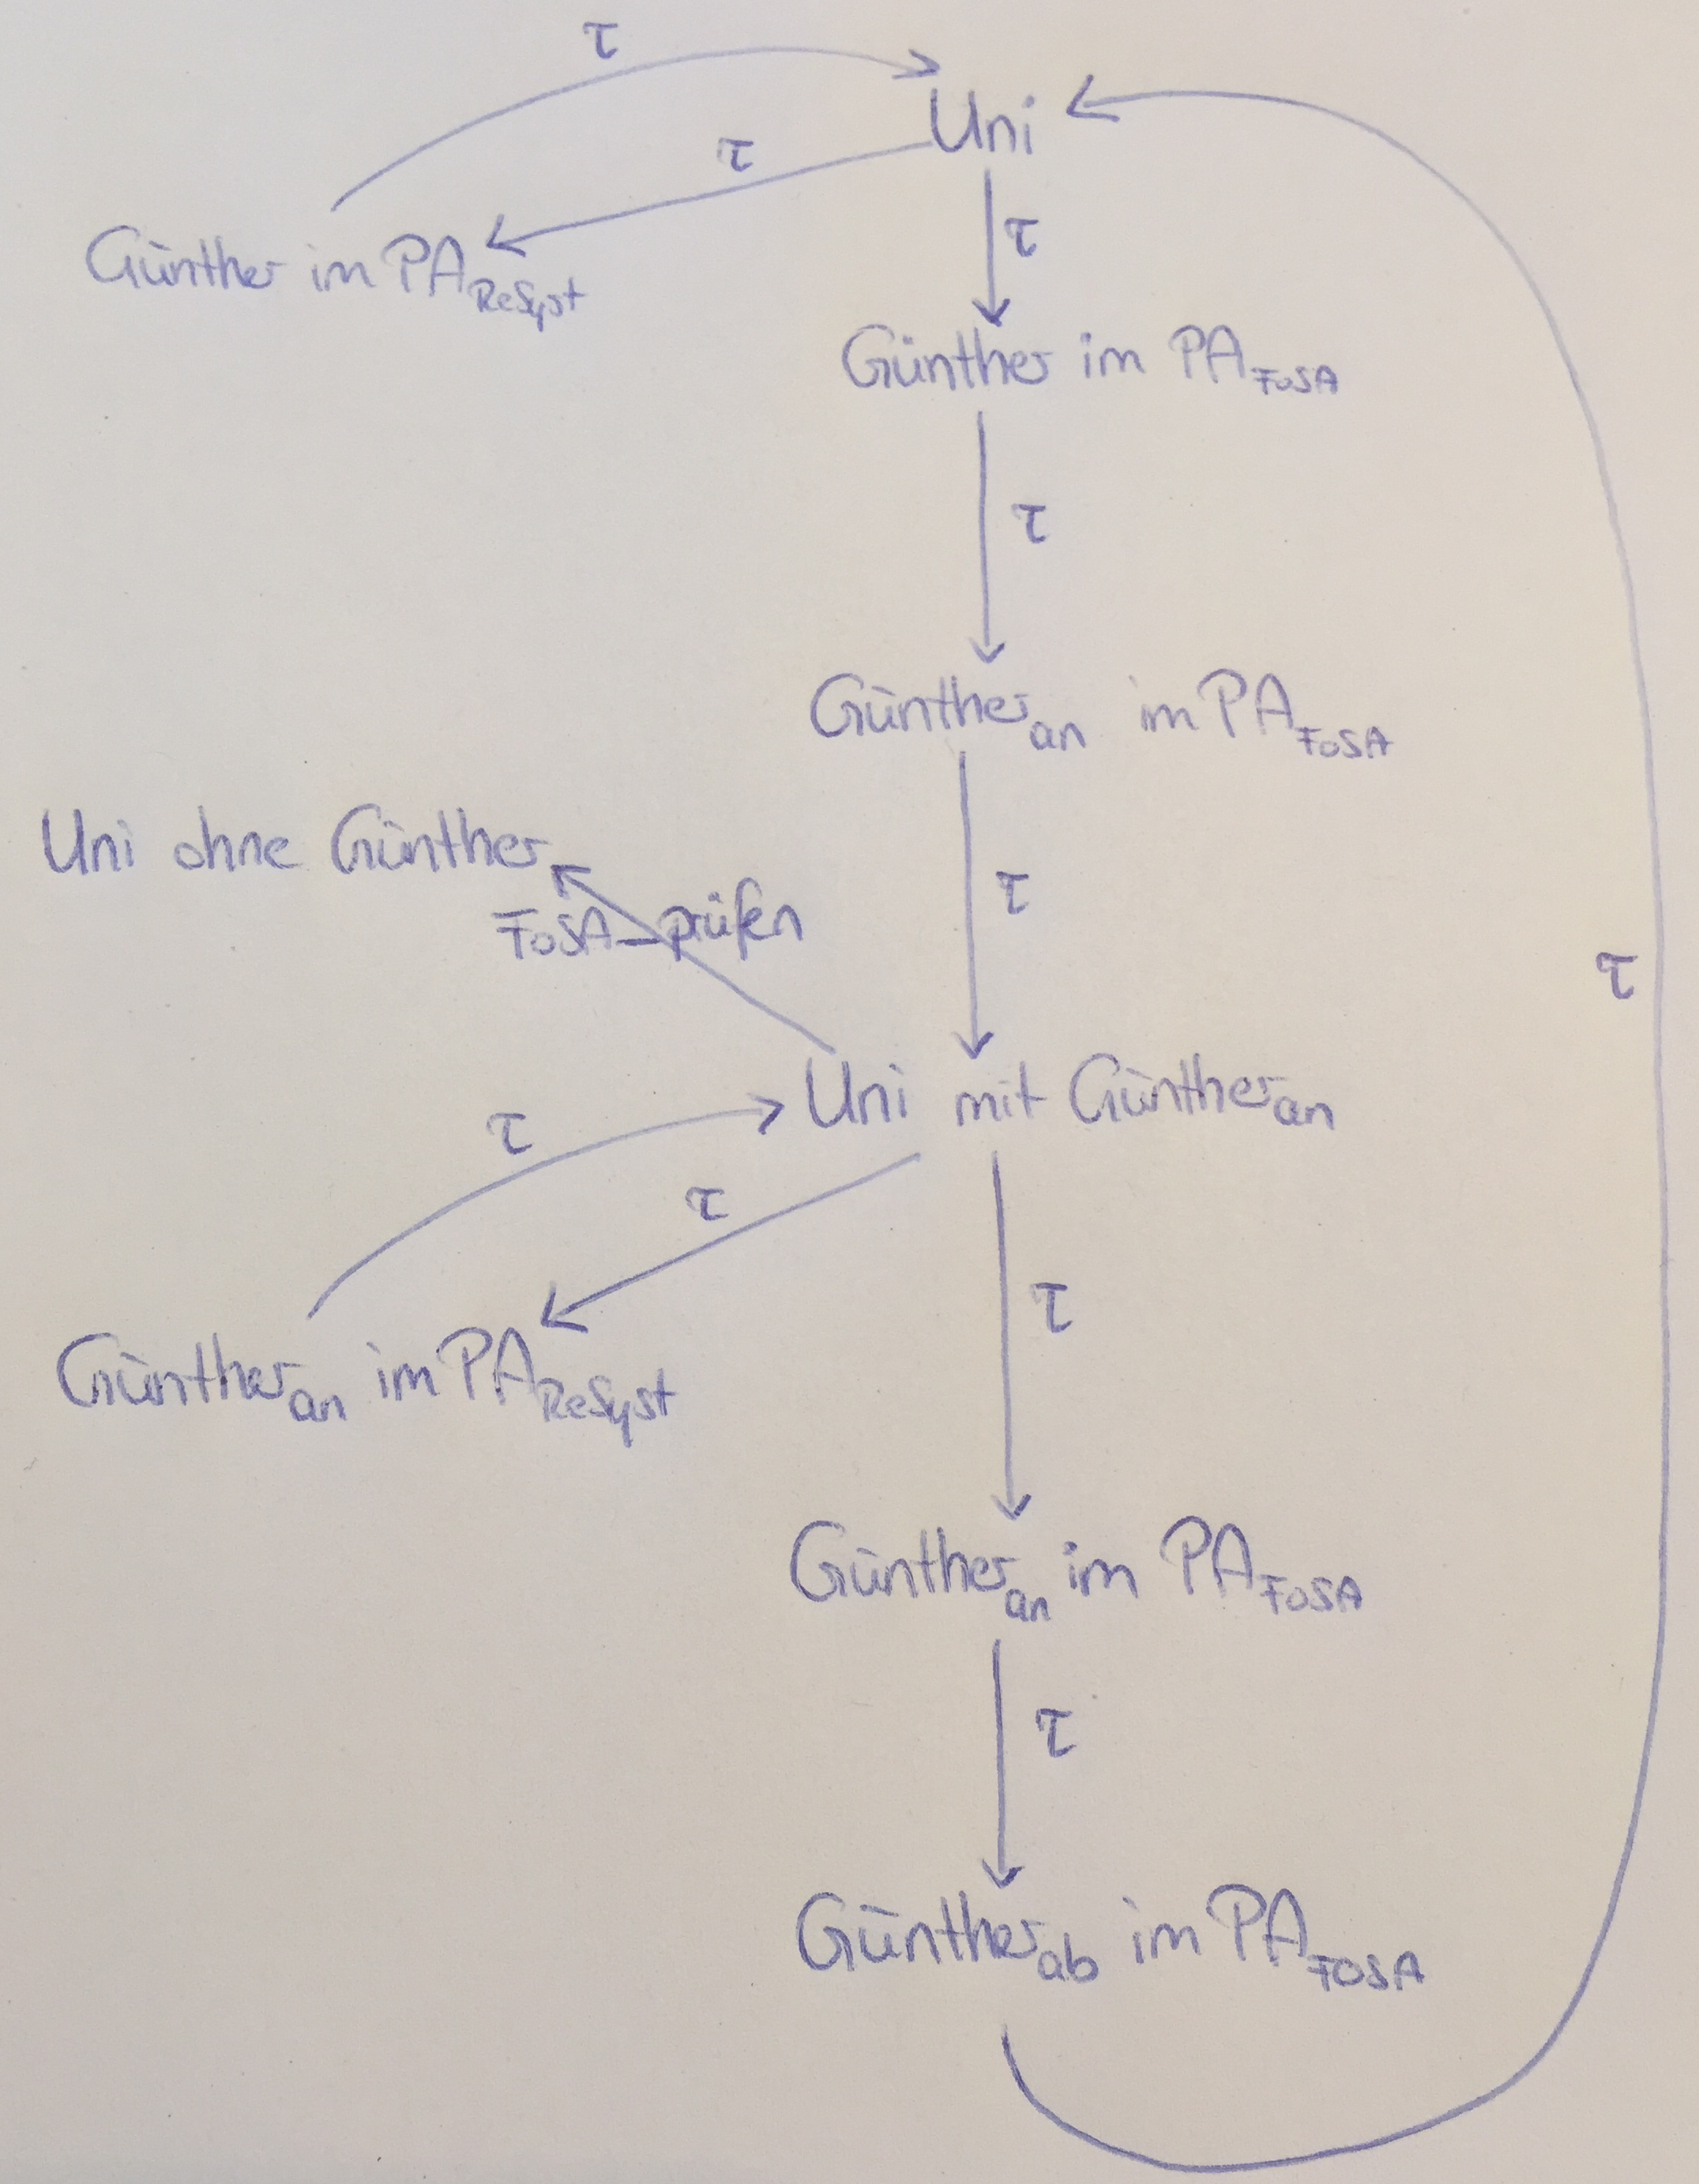
\includegraphics[width=\textwidth]{aufgabe1.png}
\end{figure}
